\apfel{} \cite{Bertone:2013vaa} is one of the most extensive tool aimed to
\pdf{}  evolution and \dis{} observables' calculation. It is provided as a
Fortran library, and it has been used by the NNPDF collaboration up to
NNPDF4.0~\cite{NNPDF:2021njg}.

\apfel{} solves \dglap{} numerically in $x$-space, sampling the evolution
kernels on a grid of points up to \nnlo{} in \qcd{}, with \qed{} evolution also
available at \lo{}.
By construction this method is \pdf{} dependent and the code is automatically
interfaced with \lhapdf{}~\cite{Buckley:2014ana}. For specific application,
the code offers also the possibility to retrieve the evolution operators
with a dedicated function.

The program supplies three different solution strategies, with various theory
setups, including scale variations and \msbar{} masses.

The stability of our benchmark at different perturbative orders is presented in \cref{fig:Apfelbench_pto},
using the settings of the Les Houches \pdf{} evolution benchmarks~\cite{Giele:2002hx,Dittmar:2005ed}.
The accuracy of our comparison is not affected by the increasing complexity
of the calculation.

\begin{figure}
    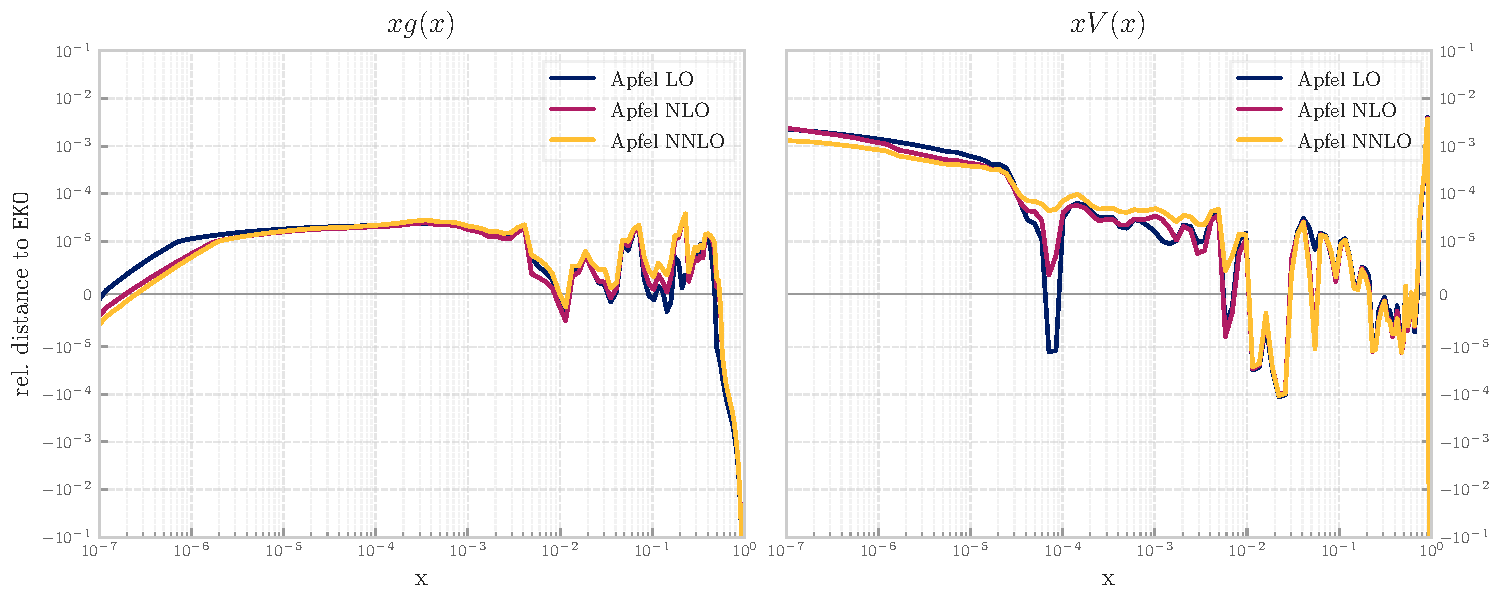
\includegraphics[width=\linewidth]{ch-eko/Apfel_bench_pto.pdf}
    \caption{Relative differences between the outcome of evolution as
        implemented in \eko{} and the corresponding results from \apfel{} at
        different perturbative orders.  We adopt the same settings of
        \cref{fig:LHAbench}.}
    \label{fig:Apfelbench_pto}
\end{figure}
